% !TEX encoding = UTF-8
% !TEX TS-program = pdflatex
% !TEX root = ../thesis.tex

%************************************************
\chapter{Hadronic Higgs Production}\label{chap:three}
%************************************************

\section{Motivation (better title needed!)}
Here I list various application for the Higgs production cross section and explain why precise predictions are so central. Maybe just put this in the chapter description?
\section{The Leading-Order Cross Section}
Having established, that the gluon-fusion Higgs production cross section is central for many phenomenological applications, we now want to perform the actual \acs{LO} calculation, which was first demonstrated by Georgi et al.\ in 1978~\cite{Georgi:1977gs}. The calculation not only serves as an instructive example on cross section calculation, and thereby allows us to put our experience from section~\ref{sec:2:cross_sections} to good use, but it already introduces many important concepts we can transfer to the \acs{NNLO} computation.

At LO, there are only two possible Feynman diagrams we can draw. They are depicted in Fig.~\ref{fig:4:LO}.
\begin{figure}[h]
\centering
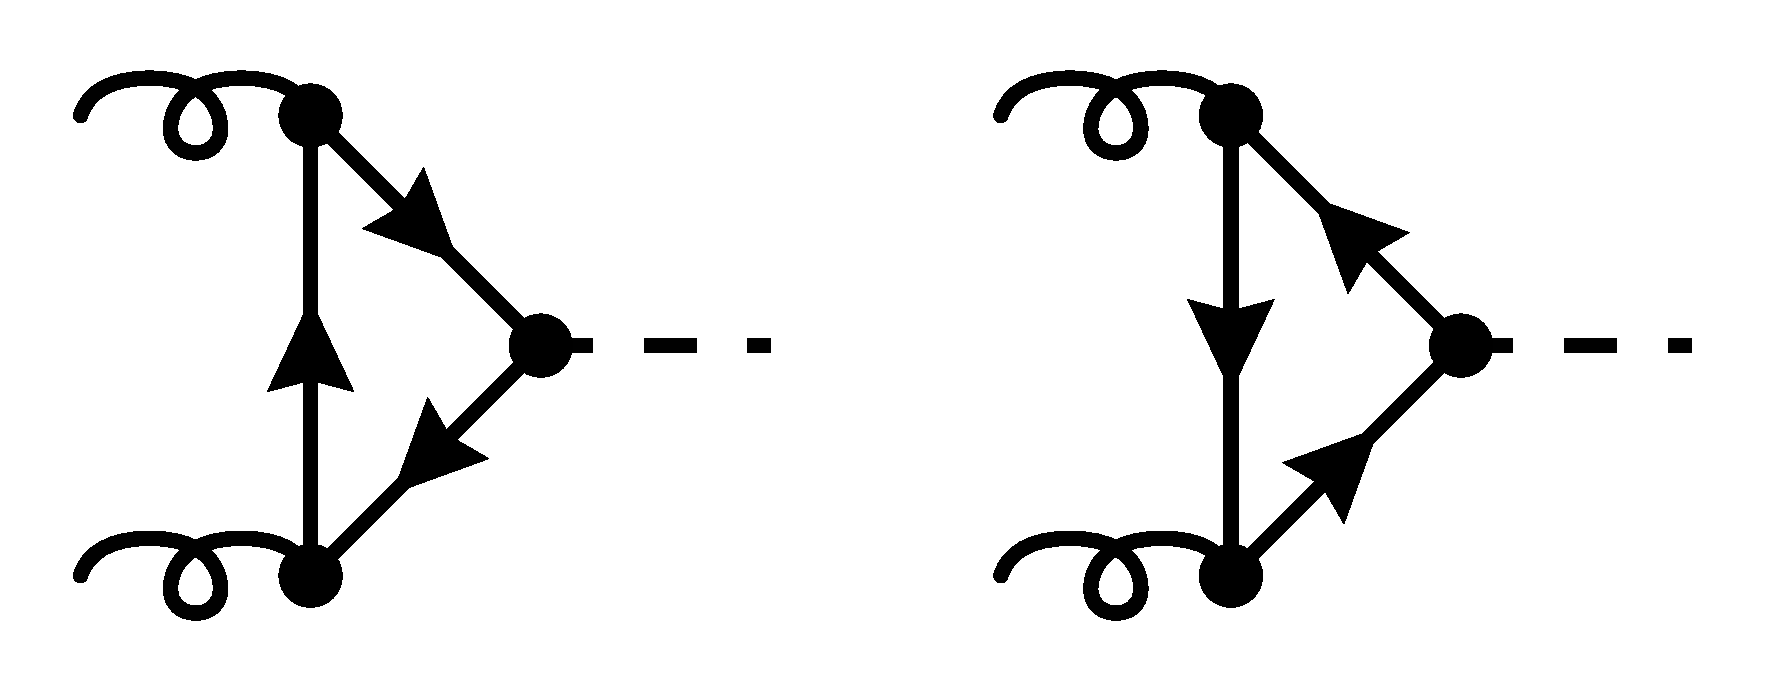
\includegraphics[scale=0.2]{Images/LO.pdf}
\caption{\acs{LO} Feynman diagrams for Higgs production in the gluon-fusion channel.}
\label{fig:4:LO}
\end{figure}
As we can see. Gluon-fusion is a loop induced process with two scales: the mass of the quark running in the loop $m_q$, and the Higgs mass $m_H$ which must simultaneously be the partonic center of mass energy. The initial state gluons carry on the on-shell momenta $p_1$ and $p_2$. Let us then define
\begin{equation}
i\mathcal{M} = i \mathcal{M}^{\mu\nu, ab} \varepsilon_\mu^a(p_1) \varepsilon_\nu^b(p_2).
\end{equation}
With the Feynman rules presented in appendix~\ref{app:1} we find
\begin{equation}
\begin{split}
&i \mathcal{M}^{\mu \nu, ab} = -\int \frac{\dd^4 k}{(2\pi)^4}\, \\
&\quad \times \text{Tr}\!\left[ \frac{-i m_q}{v} \delta_{ij} \frac{i(\slashed{k} + \slashed{p}_1 + \slashed{p}_2 + m_q)}{(k + p_1 + p_2)^2 - m_q^2} (ig \gamma^\nu T^a_{ik}) \frac{i (\slashed{k} + \slashed{p}_1 + m_q)}{(k + p_1)^2 - m_q^2} (i g \gamma^\mu T^b_{kj}) \frac{i (\slashed{k} + m_q)}{k^2 - m_q^2} \right] \\
&\quad + \lbrace p_1 \longleftrightarrow p_2,  \mu \longleftrightarrow \nu, a \longleftrightarrow b \rbrace ,
\label{eq:4:form_factor_amplitude}
\end{split}
\end{equation}
where the extra minus sign in front stems from the fermion trace.

Even without performing the explicit calculation can we already anticipate the general structure of the amplitude. Color wise, the amplitude must be proportional to $\delta^{ab}$, because it is the only available rank-two tensor. Since it is symmetric, the Lorentz structure must also be symmetric in order to satisfy \textit{Bose symmetry}. The only building blocks we have available are $g^{\mu\nu}$, $(p_1^\mu p_2^\nu + p_2^\mu p_1^\nu)$, $p_1^\mu p_1^\nu$, and $p_2^\mu p_2^\nu$, but since all transverse parts drop out of the physical amplitude, the relevant tensors are only $g^{\mu \nu}$ and $p_2^\mu p_1^\nu$. Lastly, we know that the amplitude must satisfy the \textit{Ward identity}, which allows us to restrict the tensor even further, such that we end up with
\begin{equation}
i \mathcal{M}^{\mu \nu, ab} = i\frac{\alphas}{\pi} \frac{1}{v} \delta^{ab} \left(p_2^\mu p_1^\nu - (p_1 \cdot p_2)g^{\mu\nu} \right) \mathcal{C}(m_H, m_q).
\label{eq:4:form_factor}
\end{equation}
Notice that we have only made use of very general properties of the amplitude. This is why the decomposition in Eq.~\eqref{eq:4:form_factor} will hold at every order of $\alphas$. The function $\mathcal{C}(m_H, m_q)$ is called the \textit{Higgs-gluon form factor}. It has mass dimension 0, \ie\ its functional dependence on $m_q$ and $m_H$ must be through a mass ratio
\begin{equation}
\mathcal{C} (m_H, m_q) = \mathcal{C}(z), \quad \text{with} \quad z \equiv \frac{m_H^2}{4 m_q^2}.
\end{equation}
The factor of $1/4$ was introduced, so that the \textit{normal threshold} is located at $z = 1$. Mathematically, this means that $z = 1$ is a solution of the \textit{Landau equations}. Physically, we can interpret the singularity as the point where we have enough energy to produce the quark pair on-shell. We can now project onto the form factor with
\begin{equation}
\mathcal{C}(z) = \frac{\pi v}{i \alphas} \frac{1}{N_c} \delta^{ab} \frac{1}{(p_1 \cdot p_2)^2 (d - 2)} \left(p_{2\,\mu} p_{1\,\nu} - (p_1 \cdot p_2) g_{\mu\nu} \right) i \mathcal{M}^{\mu \nu, ab}.
\end{equation}
If we now insert the \acs{LO} expression of Eq.~\eqref{eq:4:form_factor_amplitude} and perform some basic manipulations we find
\begin{equation}
\begin{split}
\mathcal{C}^{(0)} (z) = T_F \frac{1}{2 - 2 \epsilon} \frac{1}{z} \int \frac{\dd^d k}{i \pi^{d/2}} \,&\frac{1}{[k^2 - m_q^2 + i0^+][(k + p_1 + p_2)^2 - m_q^2 + i0^+]} \\
& \times \left( 2 \epsilon + \frac{m_H^2}{[(k + p_1)^2 - m_q^2 + i0^+]} \left(\frac{1}{z} + \epsilon - 1 \right) \right),
\label{eq:4:C0_integral_form}
\end{split}
\end{equation}
which, after inserting integrals and expanding in $\epsilon$, finally reduces to
\begin{equation}
\mathcal{C}^{(0)}(z) = T_F \frac{1}{z} \bigg \lbrace 1 - \left(1 - \frac{1}{z} \right) \left[ \frac{1}{2} \ln\! \left( \frac{\sqrt{1 - 1/z} - 1}{\sqrt{1 - 1/z} + 1} \right) \right]^2 \bigg \rbrace.
\end{equation}
We see that the Higgs-gluon form factor is roughly proportional to the square of the mass of the quark running in the loop. One power of $m_q$ is hereby picked up from the Yukawa coupling. The other factor $m_q$ is a consequence of the scalar coupling to Higgs. Indeed, without the quark mass, the trace in Eq.~\eqref{eq:4:form_factor_amplitude} would contain an odd number of gamma matrices and vanish consequently. Physically, we can interpret this as a helicity flip of the internal quark at the Higgs interaction vertex. And since massless \acs{QCD} conserves helicity, the other helicity flip is provided by the mass. Similarly, since the two incoming gluons are vector bosons which should form a spinless final state, we would expect them to always carry opposite spins. This intuition is indeed confirmed by the tensor structure of the amplitude \eqref{eq:4:form_factor}, as it always vanishes once contracted with two polarization vectors of the same helicity\footnote{This can be seen easily by boosting to the center of mass frame and using $\epsilon^\mu (-\mathbf{p}, \lambda) \propto \epsilon^\mu (\mathbf{p}, -\lambda)$.}.

The \acs{LO} Higgs-gluon form factor is plotted in Fig.~\ref{fig:4:form_factor}.
\begin{figure}[h]
\centering
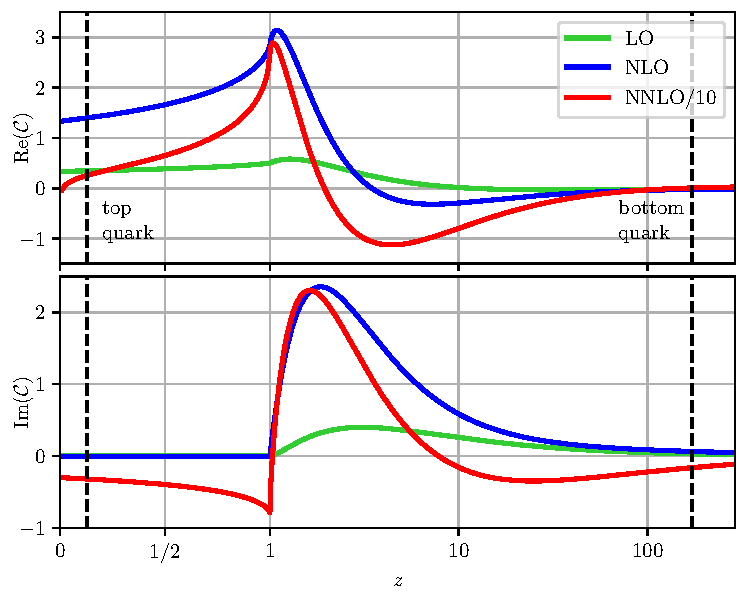
\includegraphics[width=\figurewidth]{Images/form_factor.pdf}
\caption{Real and imaginary part of the finite part of the Higgs-gluon form factor at various perturbative orders. \acs{NNLO} is divided by ten for better visibility. \acs{NNLO} results also depend on the number of light quark flavors, which has been set to 5 (5\acs{FS}). Vertical lines indicate the $z$ values for the top and bottom quark masses. The plot was created using the results of Ref.~\cite{Czakon:2020vql}.}
\label{fig:4:form_factor}
\end{figure}
As expected, we pick up an imaginary part starting from the normal threshold at $z=1$. If we expand the form factor around large quark masses, \ie\ we perform a \textit{large mass expansion} (\acs{LME}), we find that it approaches a constant
\begin{equation}
\mathcal{C}^{(0)}(z) = T_F \left( \frac{2}{3} + \frac{7}{45} z + \frac{4}{63} z^2 + \BigO{z^3} \right).
\label{eq:4:LME}
\end{equation}
We will discuss the infinite mass limit in more detail in section~\ref{sec:4:HTL}. On the other side of the spectrum we can see that if the mass of the Higgs is far greater than the mass the internal quark, the form factor is approximately
\begin{equation}
\mathcal{C}^{(0)}(z) = \frac{T_F}{4z} \left[ 4 - \log^2\!\left(-4 z \right) + \frac{1}{z} \left( \log\!\left(-4 z \right) + \log^2\!\left(-4 z \right) \right) + \BigO{1/z^2} \right].
\end{equation}
This expansion is known as \textit{high-energy limit} \acs{HEL}. The appearing double logarithms $\log^2 (m_q^2/m_H^2)$ originate from a soft quark exchange. In fact, the quark mass acts as an infrared regulator of the integral in Eq.~\ref{eq:4:C0_integral_form}, so the appearance of these logarithms is not entirely unexpected. Numerically, these logarithms can be very large. The bottom quark, for example will yield a double logarithm of about $46$. \Ie, although suppressed by a factor of $m_q^2/m_H^2$, the contributions from lighter quark flavors are logarithmically enhanced and hence highly significant for precision predictions.

If we now apply Eq.~\eqref{eq:2:Xsec} and perform the phase space integration, which for a single particle is trivial because of the momentum conserving delta function, we get for the partonic cross section
\begin{equation}
\hat{\sigma}_{gg \rightarrow H}(\tau S) = \frac{\pi}{64 v^2} m_H^2 \left( \frac{\alphas}{\pi} \right)^2 |\mathcal{C}(z)|^2 \delta\! \left(\tau S - m_H^2 \right).
\end{equation}
The initial state was averaged over spin and color. Finally, after the convolution with the partonic luminosity we arrive at the LO cross section
\begin{equation}
\sigma_{ggH}^{\text{LO}}(S) = \frac{\pi}{64v^2} \left(\frac{\alphas}{\pi} \right)^2 \mathcal{L}_{gg}\!\left(\frac{m_H^2}{S} \right) |\mathcal{C}^{(0)}(z)|^2.
\end{equation}
From Fig.~\ref{fig:4:form_factor} we can see that the top quark exerts the largest impact on the Higgs-gluon form factor and hence the \acs{LO} hadron cross section. We can read off the partonic luminosity from Fig.~\ref{fig:2:luminosity} and find that the cross section for the top quark induces Higgs production reads\footnote{Values of masses and coupling constants are provided in the \hyperref[chap:notation_and_conventions]{conventions}.}
\begin{equation}
\sigma_{ggH}^{\text{LO}} (t) = 16.30\ \GeV
\end{equation}
at a hadronic center of mass energy of $13\ \text{TeV}$. Although expected to have little impact, we can also include the effects of finite bottom quark masses by coherently summing together the corresponding form factors. We find
\begin{equation}
\sigma_{ggH}^{\text{LO}}(t+b) = 14.72\ \GeV,
\end{equation}
\ie\ the bottom quark lowers the cross section by around $9\%$ at \acs{LO}.

Without the inclusion of electro-weak corrections, we can always decompose the gluon fusion cross section in terms of the Yukawa couplings $Y_i$:
\begin{equation}
\sigma_{ggH} =  \sum_{i\le j} Y_i Y_j \sigma_{i j}.
\end{equation}
We call
\begin{equation}
\sigma_{i \times j} = Y_i Y_j \sigma_{ij},
\end{equation}
the \textit{i-j-interference contribution} and
\begin{equation}
\sigma_{i} = Y_i^2 \sigma_{ii}
\end{equation}
the \textit{pure-i contribution} to the cross section. Both contributions are depicted at \acs{LO} in Fig.~\ref{fig:4:quark_effects}.
\begin{figure}[h]
\centering
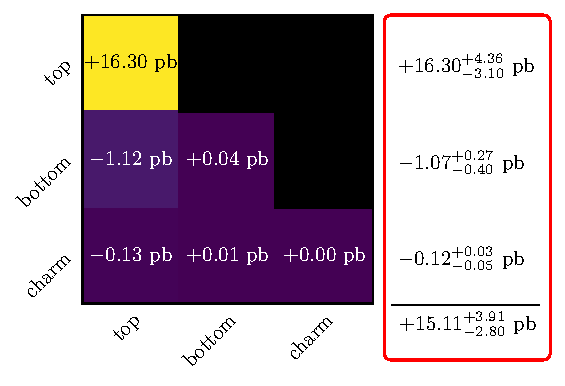
\includegraphics[scale=0.9]{Images/quark_effects_LO.pdf}
\caption{$\sigma_{i}$ (diagonals) and $\sigma_{i \times j}$ (off-diagonals) at \acs{LO} for the three heaviest quark flavors. The red box indicates the sum of each row, and hence the combined effects of each additional flavor. Computational setup is described in the \hyperref[chap:notation_and_conventions]{conventions}}
\label{fig:4:quark_effects}
\end{figure}
Clearly, the dominant contribution for the lighter quark flavors comes from the interference with the top-quark. The pure-bottom contribution is already below a percent and the pure-charm quark mass effects are completely negligible. The inclusion of the charm quark lowers the total cross section by around $2\%$, making it relevant for high precision predictions.


\section{The Heavy-Top Limit} \label{sec:4:HTL}
The computation of the Higgs production cross section in full \acs{QCD} is quite challenging. As we saw above, even at leading order we encounter loop integrals with two mass scales. It is therefore maybe not surprising that the first \acs{NLO} corrections to this process were actually computed in an approximation framework~\cite{Dawson:1990zj}. In the approximation, we assume that the quark, which is coupling to the Higgs is infinitely heavy. That means we are only interested in the leading term of the \acs{LME}.

The finite distance interaction of the gluon and the Higgs will therefore shrink down to a point like vertex, which we can describe with the effective Lagrangian
\begin{equation}
\mathcal{L}_{\text{HTL}}^{(0)} = \mathcal{L}_{\text{QCD}}^{(n_f - 1)} + \frac{\alphas}{\pi} C^{(0)} \frac{H}{v} \frac{1}{4} G^a_{\mu \nu} G^{a\, \mu\nu}.
\label{eq:4:HTL_lagrangian}
\end{equation}
We see that the coupling constant now has mass dimension $-1$, so the theory will not be \acs{UV} renormalizable. That means that we cannot absorb all \acs{UV} divergences into multiplicative renormalization constants as we did for the \acs{SM} (see Eq.~\eqref{eq:2:renormalization}), but we will generate more and more independent terms in our Lagrangian to cancel all appearing divergences. On the other hand, as long as we restrict ourselves to \acs{QCD} corrections, and hence only single operator insertions, we can treat the color singlet Higgs as a constant, and renormalize only the gauge invariant operator
\begin{equation}
\mathcal{O}_1 \equiv - 1/4 G_{\mu\nu}^a G^{a\, \mu\nu}.
\end{equation}
To indicate the pertubative order we gave the Lagrangian in Eq.~\eqref{eq:4:HTL_lagrangian} a superscript. The superscript $n_f - 1$ of the QCD Lagrangian specifies the number of active flavors. It was reduced by one, since the heaviest quark flavor was integrated out. The constant $C^{(0)}$ is called a \textit{Wilson coefficient}, and it needs to be matched to the full theory in the infinite quark mass limit. At \acs{LO} for example, we find that the Higgs-gluon form factor in the effective theory simply reads
\begin{equation}
\mathcal{C}^{(0)} = C^{(0)}.
\end{equation}
If we compare this to the leading term of our \acs{LME}~\eqref{eq:4:LME}, we find
\begin{equation}
C^{(0)} = \frac{2}{3} T_F.
\end{equation}

The main benefit of the approximation lies in the reduced complexity. By integrating out the top quark, we have reduced a loop-induced process to a tree-level process. Moreover, the top-quark mass is eliminated as a scale, hence the appearing Feynman integrals will generally be much simpler to solve.

Beyond \acs{LO} gauge invariant operator like $\mathcal{O}_1$ can mix under renormalization with other gauge invariant operators but notably also with operators which are not gauge invariant. In general, we distinguish two types of operators: \textit{Type-II operators}, which give zero when sandwiched between physical states, and \textit{type-I operators}, which can give non-zero matrix elements. The type-II operators can be further subcategorized into operators vanishing by the equation of motion (\textit{type-II${}_a$ operators}), and all other operators (\textit{type-II${}_b$ operators}). For a polynomial operator with ghost number zero satisfying
\begin{equation}
s \mathcal{O} = 0,
\end{equation}
where $s$ is the \textit{linearized Slavnov operator}, one can proof~\cite{Kluberg-Stern:1974iel, Joglekar:1975nu, Henneaux:2011rma} that
\begin{equation}
\mathcal{O} = s F + \text{gauge invariant operators}.
\end{equation}
Operators of the form $s F$ are also called \textit{Bechi-Rouet-Stora-Tyutin-} (BRST-) \textit{exact operators}, and they vanish between physical states. For $\mathcal{O}_1$ the above conditions are met, allowing us to conclude that the $\mathcal{O}_{II}$ operators are BRST-exact. This can be leveraged to find the complete operator basis:
\begin{equation}
\begin{split}
\mathcal{O}_{I} &\begin{cases} &\mathcal{O}_1 = -\frac{1}{4} G^a_{\mu \nu} G^{a\, \mu\nu}, \\
&\mathcal{O}_2 = m_q \bar{q} q, \end{cases} \\
\mathcal{O}_{II_a} &\begin{cases} &\mathcal{O}_3 = \bar{q} \left( \frac{i}{2} \overleftrightarrow{\slashed{D}} - m \right) q, \end{cases} \\
\mathcal{O}_{II_b} &\begin{cases} &\mathcal{O}_4 = A^{a\, \mu} D^\nu F_{\nu\mu}^a + g \bar{q} \slashed{A} q - \partial^\mu \bar{c}^a \partial_\mu c^a, \\
&\mathcal{O}_5 = D_\mu \partial^\mu \bar{c}^a c^a. \end{cases}
\end{split}
\label{eq:4:operators}
\end{equation}

Since operators of type II cannot generate non-vanishing $S$-matrix elements through renormalization the renormalization matrix must have the general structure
\begin{equation}
\begin{pmatrix}
\mathcal{O}_{I}^R \\
\mathcal{O}_{II}^R
\end{pmatrix} = \begin{pmatrix}
z^{I,I} & z^{I,II} \\
0 & z^{II,II}
\end{pmatrix} \begin{pmatrix}
\mathcal{O}_{I}^B \\
\mathcal{O}_{II}^B
\end{pmatrix}.
\label{eq:4:renormalization_matrix}
\end{equation}
The final form of our effective Lagrangian therefore reads
\begin{equation}
\mathcal{L}_{\text{HTL}} = \mathcal{L}_{\text{QCD}}^{(5)} + \frac{\alphas}{\pi} \frac{H}{v} \sum_{i} C_i^B \mathcal{O}_i^B.
\label{eq:4:lagrangian_operator_basis}
\end{equation}
As usual, we replace the bare quantities by their renormalized counter parts
\begin{equation}
C_i^B \mathcal{O}_i^B = C_i^B  Z_{ij}^{-1} \mathcal{O}_j^R,
\end{equation}
and we identify
\begin{equation}
C^R = (Z^{-1})^T C^B.
\end{equation}
Using the \acs{RGE} we find that the \textit{anomalous dimension} matrix of the Wilson coefficients is determined through
\begin{equation}
\frac{\dd C^R}{\dd \ln \mu} = \left(Z \frac{\dd (Z^{-1})}{\dd \ln \mu} \right)^T  C^R = - \left( \frac{\dd Z}{\dd \ln \mu} Z^{-1} \right)^T \equiv \gamma^T C^R .
\label{eq:4:anomalous_dimension_matrix}
\end{equation}
With the structure of the renormalization matrix~\eqref{eq:4:renormalization_matrix}, we arrive at an important conclusion: The Wilson coefficients of type-II operators cannot mix into the Wilson coefficients of type-I operators through the running in the scale. Since the type-II operators render no contribution to the scattering matrix element, we can focus our attention on the gauge invariant operators and their Wilson coefficients.

We now want to determine the $I,I$ part of the renormalization matrix, \ie\ $z^{I,I}$ to determine the running of the Wilson coefficients. Let us start by defining the generating functional
\begin{equation}
\begin{gathered}
Z[J] \equiv z[J]/z[0], \quad z[J] \equiv \int \prod_i \mathcal{D} \Phi_j\, e^{i(S + J \cdot \Phi)}, \quad S = S[A, c, \bar{c}, q, \bar{q}] \equiv \int \dd^d x\, \mathcal{L}, \\
J = \left( J^\mu, \bar{J}, J, \bar{\eta}, \eta \right), \quad \Phi = \left(\frac{1}{g} A_\mu, c, \bar{c}, q, \bar{q}\right),
\end{gathered}
\end{equation}
with the Lagrangian
\begin{equation}
\mathcal{L} \equiv -\frac{1}{4g^2} F^a_{\mu\nu} F^{a \, \mu \nu} - \frac{1}{2 \xi g^2} \left(\partial \cdot A \right)^2 + \partial^\mu \bar{c}^a D_\mu c^a + \bar{q} \left(\frac{i}{2} \overleftrightarrow{\slashed{D}} - m_q \right) q.
\end{equation}
The Lagrangian is the QCD Lagrangian with only one active quark flavor and rescaled gauge fields
\begin{equation}
A^a_\mu \longrightarrow \frac{1}{g} A^a_\mu.
\end{equation}
The operators in Eq.~\eqref{eq:4:operators} can now be generated by applying the differential operators\footnote{We only provide the operators for the type-I operators, since they are the only ones necessary for computing physical amplitudes. }
\begin{equation}
\begin{split}
&D_1 = - \frac{1}{2}g \frac{\partial}{\partial g} + \xi \frac{\partial}{\partial \xi} - \frac{1}{2} J_\mu \cdot \frac{\delta}{\delta J_\mu}, \\
&D_2 = - m_q \frac{\partial}{\partial m_q}, \\
\end{split}
\label{eq:4:differential_operators}
\end{equation}
on the generating functional
\begin{equation}
z_{\mathcal{O}_k}[J] \equiv \int \prod_j \mathcal{D} \Phi_j \, \hat{\mathcal{O}}_k(0) e^{i(S + J \cdot \Phi)} = - i D_k z[J].
\end{equation}
Here $\hat{\mathcal{O}}_k(0)$ is the Fourier transform of the operator $\mathcal{O}(x)$ at zero momentum. The normalization of the generating functional then properly subtracts the vacuum expectation value of the operators
\begin{equation}
-i D_k Z[J] = \frac{1}{z[0]}\int \prod_j \mathcal{D} \Phi_j \, \left(\hat{\mathcal{O}}_k(0) - \braket{\Omega | \mathcal{O}_k(0) |\Omega} \right) e^{i (S + J \cdot \Phi)} \equiv Z_{\mathcal{O}_k}.
\end{equation}
In the \MS\ scheme, the $R$-operation commutes with the differential operators in Eq.~\eqref{eq:4:differential_operators}, \ie\ the renormalized operators can be generated from the renormalized generating functional
\begin{equation}
Z_{\mathcal{O}_k^R} = -i D_k Z^R[J],
\end{equation}
where the renormalized generating functional is defined as
\begin{equation}
\begin{gathered}
Z^R[J] = z^R[J]/z^R[0] ,\\
\quad z^R[J] = \int \prod_i \mathcal{D}\Phi_j \, e^{i(S^R + J \cdot \Phi)}, \\
S^R \equiv S[Z_3^{\prime\, 1/2} A^R, Z_3^{\prime\, -1/2} c^R, \tilde{Z}_3^{-1/2}\bar{c}^R, Z_2^{1/2} q^R, Z_2^{1/2} \bar{q}^R, Z_g g, Z_m m_q, Z_g^{-2} Z_3^\prime \xi^R].
\end{gathered}
\end{equation}
Using the chain rule we find that
\begin{equation}
-i D_k z^R[J] = \int \prod_j \mathcal{D} \Phi_j \, \left[ \hat{O}_k(0) + \sum_i (D_k \ln Z_i)  \frac{\partial S^R}{\partial \ln Z_i}\right] e^{i S^R + J \cdot \Phi}, \quad Z_i \in \big \lbrace Z_3^\prime , \tilde{Z}_3, Z_2, Z_g, Z_m \big \rbrace.
\end{equation}
And with
\begin{equation}
Z_g \frac{\partial S^R}{\partial Z_g} = - 2 \hat{\mathcal{O}}_1(0), \quad \text{and} \quad Z_m \frac{\partial S^R}{\partial Z_m} = - \hat{\mathcal{O}}_2(0),
\end{equation}
we find that the renormalization constants are given by
\begin{equation}
\begin{alignedat}{2}
&z^{I,I}_{11} = 1 - 2 D_1 \ln Z_g = 1 + g\frac{\partial \ln Z_g}{\partial g}, \quad &&z^{I,I}_{12} = - D_1 \ln Z_m = \frac{g}{2} \frac{\partial \ln Z_m}{\partial g} \\
&z^{I,I}_{21} = 0, \quad &&z^{I,I}_{22} = 1.
\end{alignedat}
\end{equation}
Here we made use of the fact, that the \MS-renormalization constants are independent of the quark mass and the gauge parameter. We can rewrite the appearing derivatives in terms of the $\beta$-function and the mass-anomalous dimension. Indeed,
\begin{equation}
\begin{gathered}
\frac{4\pi}{\alphas} \bar{\beta} \equiv \frac{\dd \ln \alphas}{\dd \ln \mu} = - \frac{\dd \ln Z_{\alphas}}{\dd \ln \mu} = - \left( \frac{\partial \ln Z_{\alphas}}{\partial \ln \alphas} \frac{\dd \ln \alphas}{\dd \ln \mu} + \frac{\partial \ln Z_{\alphas}}{\partial \ln\mu} \right) = - \left(  \frac{\bar{\beta}}{\alphas} \frac{\partial \ln Z_{\alphas}}{\partial \ln \alphas} + 2 \epsilon \right) \\
\Rightarrow \frac{\partial \ln Z_{\alphas}}{\partial \ln \alphas} = g \frac{\partial \ln Z_g}{\partial g} = - 4\pi - 2 \epsilon \frac{\alphas}{\bar{\beta}} = -1 + \frac{1}{1 - \frac{\beta}{2 \epsilon} \frac{4 \pi}{\alphas}},
\end{gathered}
\end{equation}
where in the last step we used the relation between the $d$- and four-dimensional $\beta$-functions
\begin{equation}
\bar{\beta} = \beta - 2 \epsilon \frac{\alphas}{4 \pi}.
\label{eq:4:d_dimensional_beta_function}
\end{equation}
Similarly, we find
\begin{equation}
\begin{gathered}
\gamma_m \equiv - \frac{\dd \ln m_q}{\dd \ln \mu} = \frac{\dd \ln Z_m}{\dd \ln \mu} = \frac{\partial \ln Z_m}{\partial \ln \alphas} \frac{\partial \ln \alphas}{\partial \ln \mu} = \frac{\partial \ln Z_m}{\partial \ln \alphas} \frac{4 \pi}{\alphas} \bar{\beta} \\
\Rightarrow \frac{\partial \ln Z_m}{ \partial \ln \alphas} = g \frac{\partial \ln Z_m}{\partial g} = \frac{\alphas}{4 \pi} \frac{1}{\bar{\beta}} \gamma_m = - \frac{\gamma_m}{2 \epsilon} \frac{1}{1 - \frac{\beta}{2 \epsilon} \frac{4 \pi}{\alphas}}
\end{gathered}
\end{equation}

Finally, we want to use the above results to calculate the anomalous dimension matrix in Eq.~\eqref{eq:4:anomalous_dimension_matrix}. The entries of the renormalization constant only depend on scale through the coupling constant, \ie\
\begin{equation}
\gamma^{I,I} = -\frac{\dd z^{I,I}}{\dd \ln \mu} (z^{I,I})^{-1} \bigg \vert_{\epsilon = 0} = -\frac{\partial z^{I,I}}{\partial \alphas} (z^{I,I})^{-1} 4 \pi \bar{\beta} \bigg \vert_{\epsilon = 0} = \frac{\partial z^{I,I\,(1)}}{\partial \alphas} 2 \alphas.
\end{equation}
Where we used that $z^{I,I}$ consists only of poles in the \MS\ scheme, and once again applied the relation between the $\beta$-functions in Eq.~\eqref{eq:4:d_dimensional_beta_function}. $z^{I,I\, (1)}$ denotes the residue of the renormalization matrix
\begin{equation}
z^{I,I} = \mathbb{1} + \sum_{i = 1} z^{I,I\,(i)} \epsilon^{-i}.
\end{equation}
We then find for the anomalous dimension matrix
\begin{equation}
\gamma^{I,I} = \begin{pmatrix} 4 \pi \alphas \frac{\dd}{\dd \alphas} \left( \frac{\beta}{\alphas} \right) & - \alphas \frac{\dd \gamma_m}{\dd \alphas} \\
0 & 0 \end{pmatrix}.
\end{equation}
The structure of this matrix reveals, that the $C_1$ Wilson coefficient, which is relevant coefficient for the  \acs{HTL}, is completely independent of the other Wilson coefficients. The \acs{RGE} for the Wilson coefficient~\eqref{eq:4:anomalous_dimension_matrix} can now be written as \
\begin{equation}
\frac{\partial C_1}{\partial \alphas} 4 \pi \beta + \frac{\partial C_1}{\partial \ln \mu} = 4 \pi \alphas \frac{\dd }{\dd \alphas} \left(\frac{\beta}{\alphas} \right).
\label{eq:4:RGE_of_C1}
\end{equation}
The $beta$-function has the general expansion
\begin{equation}
\beta = \left(\frac{\alphas}{4 \pi} \right)^2 \sum_{i = 0} \beta_i \left(\frac{\alphas}{4 \pi} \right)^i.
\end{equation}
For example at one-, and two-loop, it can be shown~\cite{Gross:1973id, Politzer:1973fx, tHooft:1972ikm, Caswell:1974gg, Jones:1974mm, Egorian:1978zx}
\begin{equation}
\begin{split}
&\beta_0 = \frac{11}{3} C_A - \frac{4}{3} T_F n_f, \\
&\beta_1 = \frac{34}{3} C_A^2 - \frac{20}{3} C_A T_F n_f - 4 C_F T_F n_f.
\end{split}
\end{equation}
We can solve the partial differential equation in Eq.~\eqref{eq:4:RGE_of_C1} perturbatively by proposing the Ansatz
\begin{equation}
\begin{split}
C_1 =  &\ C_1^{(0,0)} + \frac{\alphas}{4 \pi} \left(C_1^{(1,0)} + C_1^{(1, 1)} \ln \frac{\mu}{\mu_0} \right) \\
&+ \left(\frac{\alphas}{4 \pi} \right)^2 \left(C_1^{(2, 0)} + C_1^{(2, 1)} \ln \frac{\mu}{\mu_0} + C_1^{(2, 2)} \ln^2 \frac{\mu}{\mu_0} \right) + \BigO{\alphas^3}.
\end{split}
\end{equation}
The constants coefficients $C_1^{(i, 0)}$ mark the initial conditions; they need to be matched to the full theory in the infinite mass limit. The coefficients of the logarithms on the other hand can be determined through a comparison of coefficients, they read
\begin{equation}
C_1^{(1,1)} = 0, \quad C_1^{(2, 1)} = C_1^{(0,0)} \beta_1 - C_1^{(1, 0)} \beta_0, \quad C_1^{(2, 2)} = 0.
\end{equation}
It is clear from the structure of the differential equation, that the all coefficients $C_1^{(i, i)}$ are in fact all zero except for $C_1^{(0,0)}$.

By expanding the Higgs-gluon form for large quark masses we were able to determine the \acs{LO} Wilson coefficient\footnote{Notice the different signs in Eqs.~\eqref{eq:4:HTL_lagrangian} and \eqref{eq:4:lagrangian_operator_basis}. So the Wilson coefficients are related by $C_1^{(0,0)} = - C^{(0)} = -\frac{2}{3}T_F$.}. Of course, if we would need the full Higgs-gluon form factor to determine the Wilson coefficient, the \acs{HTL} would be of little use, since it would not bring any simplifications. Fortunately, the large quark mass limit can already be used at the integrand level using the large mass expansion,



\section{Higher-Order Corrections}
Here I outline how to perform higher order corrections.
\section{Theory Status}
Here I describe what is already known about the gluon-gluon fusion channel. I explain the theory uncertainties.

